52. \begin{figure}[ht!]
\center{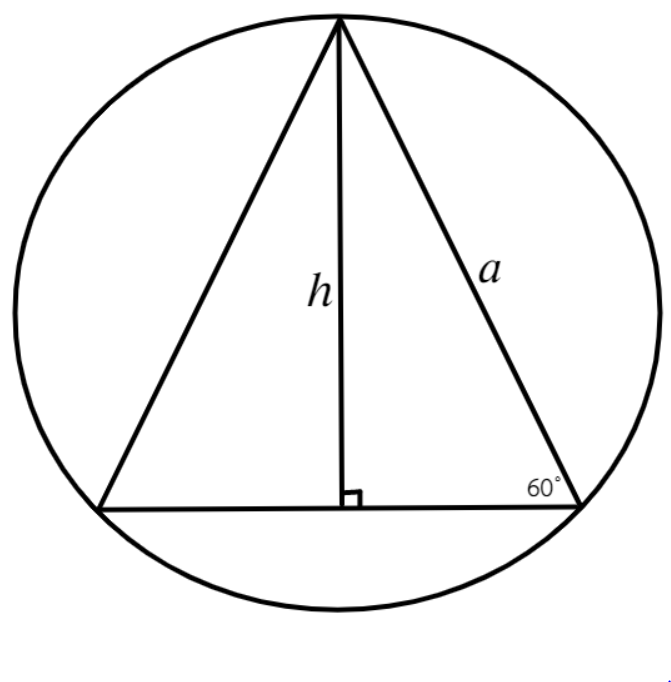
\includegraphics[scale=0.35]{g9-52.png}}
\end{figure}\\
Пусть сторона правильно треугольника равна $a,$ а высота $h.$ По теореме синусов имеем соотношение $\cfrac{a}{\sin(60^\circ)}=2R,\ a=\cfrac{\sqrt{3}}{2}\cdot\sqrt{12},\ a=3.$ Тогда высота $h=a\sin(60^\circ)=3\cdot\cfrac{\sqrt{3}}{2}=\cfrac{3\sqrt{3}}{2}.$ Радиус вписанной окружности равностороннего треугольника можно найти по формуле $r=\cfrac{h}{2}tg(30^\circ)=\cfrac{3\sqrt{3}}{4}\cdot\cfrac{\sqrt{3}}{3}=\cfrac{3}{4}.$\\
